\chapter{希格斯机制：规范玻色子如何获得质量}

现在我们把上一讲中发展出的两个想法结合起来。一个具有破缺的整体\(U(1)\)对称性的复标量场，包含一个有质量的径向振荡和一个无质量的角向振荡。一个局域不变的\(U(1)\)理论包含一个无质量的规范场。当标量带荷且其平衡幅度非零时，这些陈述不能简单地相加。角向模式与规范场结合：规范场获得质量，表观的戈德斯通玻色子不再是独立粒子，而径向的希格斯模式仍然保留。

光子将作为我们的模型规范玻色子，但不是我们的物理结论。电磁\(U(1)\)在真空中并未破缺，因此真实的光子是无质量的。同一机制作用于电弱理论中的\(W^\pm\)和\(Z\)，在那里规范群和标量多重态更为复杂。阿贝尔模型揭示了这一机制，而没有把它隐藏在群论之下。

\begin{classroomqa}
\audiencequestion{先前的讨论是否意味着希格斯机制赋予真实光子以质量？\lecturetimestamp{00:00:23}}
\lecturerresponse{不。我们问的是，\emph{如果}与光子相关的\(U(1)\)处于破缺相，会发生什么。那个假想的光子会获得质量。真实的电磁真空并不处于该相；对粒子物理的应用反而是\(W\)和\(Z\)的质量。}
\end{classroomqa}

与电荷守恒相关的对称性是相位旋转
\begin{equation}
  \phi(x)\longmapsto e^{i\theta}\phi(x),
\end{equation}
一种称为\(U(1)\)的内部旋转。超导体提供了破缺相的一个真实类比。在其内部，电磁场具有有限的穿透深度，并在重要方面表现得像一个有质量的场。在其外部，普通无质量的光子重新出现。

\section{质量对场意味着什么}

\subsection{色散与零动量能隙}

在引入希格斯场之前，值得精确地确定我们所说的质量是什么意思。对于波，
\begin{equation}
  E=\hbar\omega,
  \qquad
  p=\hbar k,
  \label{eq:l08-quantum-wave}
\end{equation}
因此\((E,p)\)图和\((\omega,k)\)图包含相同的信息，只差\(\hbar\)的因子。在真空中，无质量的相对论性激发满足
\begin{equation}
  E=c|p|,
  \qquad
  \omega=c|k|.
  \label{eq:l08-massless-dispersion}
\end{equation}
\(k\)的两个符号区分相反的传播方向。要点在于\(\omega\)随\(k\)趋于零。

有质量的相对论性粒子满足
\begin{equation}
  E^2=c^2p^2+m^2c^4.
  \label{eq:l08-massive-dispersion}
\end{equation}
在单位\(c=\hbar=1\)下，
\begin{equation}
  \omega^2=k^2+m^2.
\end{equation}
在\(k=0\)处，能量为\(E=mc^2\)，或在自然单位下简写为\(m\)。因此质量是零动量模式非零的能量间隙。

\begin{figure}[htbp]
\centering
\begin{adjustbox}{max width=\linewidth}
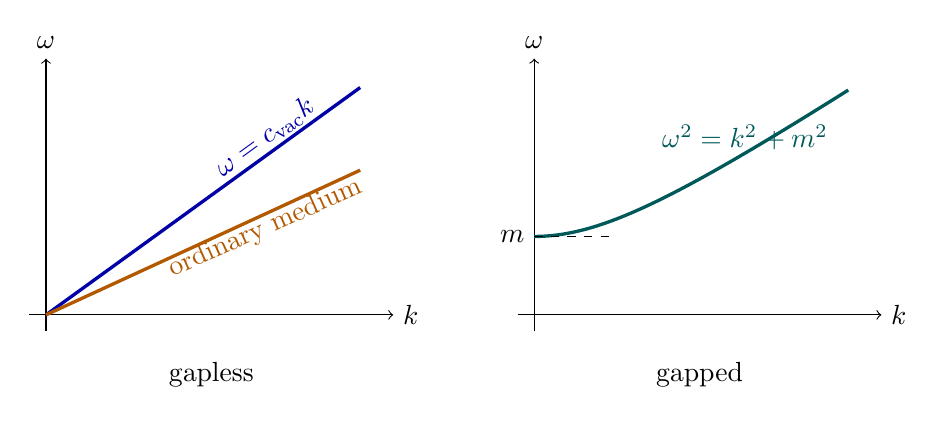
\begin{tikzpicture}[x=1.05cm,y=1.05cm]
  \begin{scope}
    \draw[->] (-0.2,0) -- (4.2,0) node[right] {\(k\)};
    \draw[->] (0,-0.2) -- (0,3.1) node[above] {\(\omega\)};
    \draw[very thick,blue!65!black] (0,0) -- (3.8,2.75);
    \draw[very thick,orange!70!black] (0,0) -- (3.8,1.75);
    \node[blue!65!black,rotate=36] at (2.65,2.15)
      {\(\omega=c_{\rm vac}k\)};
    \node[orange!70!black,rotate=24] at (2.65,1.05)
      {ordinary medium};
    \node[below] at (2,-0.45) {gapless};
  \end{scope}
  \begin{scope}[xshift=6.2cm]
    \draw[->] (-0.2,0) -- (4.2,0) node[right] {\(k\)};
    \draw[->] (0,-0.2) -- (0,3.1) node[above] {\(\omega\)};
    \draw[very thick,domain=0:3.8,samples=120,smooth,teal!70!black]
      plot (\x,{sqrt(0.9+0.45*\x*\x)});
    \draw[dashed] (0,0.95) -- (1.0,0.95);
    \node[left] at (0,0.95) {\(m\)};
    \node[teal!70!black] at (2.55,2.15)
      {\(\omega^2=k^2+m^2\)};
    \node[below] at (2,-0.45) {gapped};
  \end{scope}
\end{tikzpicture}
\end{adjustbox}
\caption{改变传播速度会改变无隙色散关系的斜率。赋予激发以质量会在\(k=0\)处打开一个非零能隙。}
\label{fig:l08-dispersion}
\end{figure}

普通透明材料可以降低波的相速度，而不产生这种相对论性质量能隙。在边界处，入射频率是固定的，而波数则按照介质的色散关系调整。改变斜率与抬高截距不是一回事。
\editorialnote{一种材料可以有若干电磁分支，而等离子体或共振介质可以具有非零的等离子体频率能隙。本讲的比较特指普通折射分支与超导响应之间。更一般地说，无隙性意味着当\(k\to0\)时\(\omega(k)\to0\)；并非每个非相对论介质都要求严格的线性。}

\begin{classroomqa}
\audiencequestion{光子每当穿过物质，例如穿过棱镜时，都会获得质量吗？\lecturetimestamp{00:03:02}}
\lecturerresponse{不。折射可以改变频率与波数之间的关系，从而改变传播速度，而该分支仍然在\(k=0\)处通过\(\omega=0\)。超导相则相反，它使电磁响应具有有限的倒数穿透长度，即质量的类比物。}
\end{classroomqa}

\begin{classroomqa}
\audiencequestion{对于固定频率的光进入玻璃，改变的是波数吗？\lecturetimestamp{00:09:20}}
\lecturerresponse{是的。静止界面处的时间平移不变性使频率保持固定。由于色散曲线在玻璃中具有不同的斜率，相同的\(\omega\)对应不同的\(k\)，因而对应不同的波长。}
\end{classroomqa}

斜率
\begin{equation}
  v_g=\frac{d\omega}{dk}
\end{equation}
是波包的群速度。如果该斜率随\(k\)变化，不同的傅里叶分量以不同的速度运动，波包便发生色散。这就是为什么关系\(\omega(k)\)被称为\emph{色散关系}。

\begin{classroomqa}
\audiencequestion{这条曲线叫什么名字，它的斜率代表什么？\lecturetimestamp{00:11:02}}
\lecturerresponse{这条曲线是色散关系。它的导数
\(d\omega/dk\) 是群速度。恒定的斜率使所有波长具有相同的速度；变化的斜率则使波包扩散。就当前目的而言，决定性的区别在于该曲线是到达原点还是存在间隙。}
\end{classroomqa}

\subsection{均匀振荡是静止的粒子}

模式 \(k=0\) 具有无限波长：场在各处被移动了相同的量。释放一个均匀位移。如果场以非零频率振荡，则相应的量子具有非零静止能量，因而有质量。如果在该方向上没有回复力，则频率为零，该模式无质量。

这一陈述是经典的。它并不要求空间上分离的粒子处于量子叠加态。均匀的经典场位形只是同一个场值在整个空间中重复。

\begin{classroomqa}
\audiencequestion{如果整个场一起被移动，这与量子纠缠相同吗？\lecturetimestamp{00:10:04}}
\lecturerresponse{不相同。均匀的经典场是一种经典位形。纠缠关联的是不同的量子备选，例如自旋向上--向下与自旋向下--向上的自旋位形。在许多点上制备相同的场值本身并不是纠缠，也不意味着瞬时因果响应。}
\end{classroomqa}

对于按正则归一化的实场，
\begin{equation}
  \mathcal L
  =\frac12\partial_\mu\varphi\,\partial^\mu\varphi-V(\varphi),
\end{equation}
在平衡点 \(\varphi_0\) 附近展开：
\begin{equation}
  V(\varphi_0+\eta)
  =V(\varphi_0)
   +\frac12V''(\varphi_0)\eta^2+\cdots.
\end{equation}
线性项在极小值处消失，场方程给出
\begin{equation}
  \omega^2=\bm{k}^2+m^2,
  \qquad
  m^2=V''(\varphi_0).
  \label{eq:l08-curvature-mass}
\end{equation}
因此，质量是势在运动方向上的曲率。平坦方向具有零曲率，并给出无质量模式。

\section{破缺的复标量}

\subsection{径向运动与角向运动}

将复标量写成笛卡儿坐标和极坐标：
\begin{equation}
  \phi=\phi_R+i\phi_I=\rho e^{i\alpha},
  \qquad
  \phi^*=\phi_R-i\phi_I=\rho e^{-i\alpha}.
  \label{eq:l08-polar-field}
\end{equation}
复平面是一个\emph{内部}场空间。在每个物理
时空点 \(x\) 处，这一对
\((\phi_R(x),\phi_I(x))\) 指定了该内部平面中的一个点。
两个内部轴都不是实验室中的方向。

\begin{figure}[htbp]
\centering
\includegraphics[width=0.72\textwidth]{lecture_08_figure_02.png}
\caption{复标量在其内部
\((\phi_R,\phi_I)\) 平面中的表示。半径是 \(\rho\)，而 \(\alpha\) 是
内部相位。}
\lectureframe{00:24:41}
\label{fig:l08-internal-plane}
\end{figure}

标量动能项变为
\begin{align}
  \partial_\mu\phi^*\,\partial^\mu\phi
  &=
  \partial_\mu\phi_R\,\partial^\mu\phi_R
  +\partial_\mu\phi_I\,\partial^\mu\phi_I
  \notag\\
  &=
  \partial_\mu\rho\,\partial^\mu\rho
  +\rho^2\partial_\mu\alpha\,\partial^\mu\alpha.
  \label{eq:l08-polar-kinetic}
\end{align}
一个全局 \(U(1)\) 不变的势依赖于
\(\phi^*\phi=\rho^2\)，而不依赖于 \(\alpha\)。例如，
\begin{equation}
  V(\phi)
  =\lambda\left(\phi^*\phi-\frac{f^2}{2}\right)^2,
  \qquad \lambda>0.
  \label{eq:l08-mexican-hat}
\end{equation}
它的极小值构成一个圆。该规律在共同的相位旋转下不变，但选择一个平衡相位就选定了该圆上的一个点。

\begin{figure}[htbp]
\centering
\includegraphics[width=0.78\textwidth]{lecture_08_figure_03.png}
\caption{黑板上的径向势草图。该势在内部场值的旋转下是对称的，尽管场本身不必位于原点。}
\lectureframe{00:34:22}
\label{fig:l08-radial-potential-board}
\end{figure}

\begin{figure}[htbp]
\centering
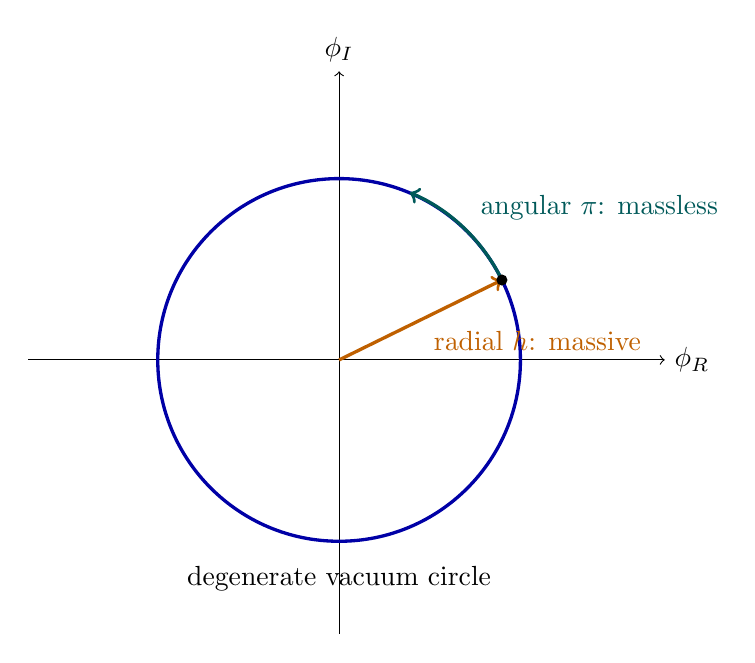
\begin{tikzpicture}[x=0.94cm,y=0.94cm]
  \draw[->] (-4.2,0) -- (4.4,0) node[right] {\(\phi_R\)};
  \draw[->] (0,-3.7) -- (0,3.9) node[above] {\(\phi_I\)};
  \draw[very thick,blue!65!black] (0,0) circle (2.45);
  \draw[->,very thick,orange!75!black] (0,0) -- (2.2,1.08);
  \draw[->,very thick,teal!70!black]
    (2.2,1.08) arc[start angle=26,end angle=67,radius=2.45];
  \node[orange!75!black,below right] at (1.15,0.52)
    {radial \(h\): massive};
  \node[teal!70!black,above right] at (1.78,1.76)
    {angular \(\pi\): massless};
  \fill (2.2,1.08) circle (2pt);
  \node[below] at (0,-2.65) {degenerate vacuum circle};
\end{tikzpicture}
\caption{全局破缺理论在垂直于真空圆的方向上有曲率，但沿该圆没有曲率。径向希格斯模式有质量；角向戈德斯通模式无质量。}
\label{fig:l08-radial-angular}
\end{figure}

令
\begin{equation}
  \phi(x)=\frac{f+h(x)}{\sqrt2}
           e^{i\pi(x)/f}.
  \label{eq:l08-canonical-polar}
\end{equation}
在所选真空附近，\(h\) 度量径向位移，而 \(\pi\)
以正则量纲度量切向位移。代入
式~\eqref{eq:l08-polar-kinetic} 给出
\begin{equation}
  \partial_\mu\phi^*\,\partial^\mu\phi
  =
  \frac12(\partial_\mu h)^2
  +\frac12\left(1+\frac{h}{f}\right)^2
            (\partial_\mu\pi)^2.
  \label{eq:l08-global-expanded}
\end{equation}
式~\eqref{eq:l08-mexican-hat} 中的势给出
\begin{equation}
  m_h^2=2\lambda f^2,
  \qquad
  m_\pi^2=0.
  \label{eq:l08-global-masses}
\end{equation}
在远低于 \(m_h\) 的能量下，径向运动代价很高，因此我们可以
暂时冻结 \(h=0\)。剩余的拉格朗日量只包含
\(\frac12(\partial\pi)^2\)，没有 \(\pi^2\) 项。这就是戈德斯通
玻色子。\editorialnote{在两处，口头解释颠倒了名称，并说吃掉戈德斯通玻色子使希格斯玻色子获得质量。黑板上的计算和本讲其余部分确立了本意结果：径向曲率已经使希格斯模式获得质量，而规范玻色子获得戈德斯通模式并变得有质量。}

\begin{classroomqa}
\audiencequestion{这是标准模型中唯一的自发对称性破缺吗？\lecturetimestamp{00:16:39}}
\lecturerresponse{电弱希格斯相是此处相关的已确立的
对称性破缺机制。其实际对称性是
\(SU(2)_L\times U(1)_Y\)，而不是这个单一的 \(U(1)\)，并且 QCD 具有额外的
真空结构，例如手征对称性破缺。这个阿贝尔例子是
规范玻色子机制的一个刻意简化的模型。}
\end{classroomqa}

\begin{classroomqa}
\audiencequestion{希格斯是否赋予每个粒子质量，包括它自身？\lecturetimestamp{00:17:11}}
\lecturerresponse{这里存在一个既是又不是的区分。电弱对称性禁止\(W\)、\(Z\)以及标准模型费米子具有裸质量；它们的质量在希格斯场取得非零平衡幅度之后才出现。径向希格斯质量来自其自身势的曲率。其他假想粒子可以拥有与这一机制无关的、对称性允许的质量。}
\end{classroomqa}

讲座将这类对称性允许的质量与可能非常重、难以观测的粒子联系起来，并提到暗物质作为一个可能的例子。那是一种动机，而不是质量预言。
\editorialnote{暗物质的质量尺度仍然未知。讲座中关于粒子质量约为质子质量一千倍的提示属于历史性推测，而不是暗物质已被实验确立的性质。}

\begin{classroomqa}
\audiencequestion{\(\rho\)是物理半径，还是场值？究竟什么才是径向对称的？\lecturetimestamp{00:33:08}}
\lecturerresponse{在每个时空点，场值是辅助复平面上的一个点，而\(\rho=|\phi|\)是该点到原点的距离。\emph{势}在这个内部平面上是径向对称的：所有具有相同\(\rho\)的点都具有相同的势能。这个半径不是普通空间中的距离。}
\end{classroomqa}

\begin{classroomqa}
\audiencequestion{足够剧烈的径向踢动能否把场带过中心极大值，到达势的另一侧？
\lecturetimestamp{00:36:00}}
\lecturerresponse{原则上，能量足够高的局域位形可以越过势垒。让一个均匀的宏观场越过它则需要巨大的能量，而一般的剧烈扰动会把能量耗散到许多场模式中，而不是相干地到达对侧点。低能近似之所以冻结\(\rho\)，正是因为在那里这种径向偏离不可及。}
\end{classroomqa}

\section{为什么复平面不是时空}

物理坐标与内部坐标之间的区分值得讲座用整整一段来停顿说明。标量场之所以称为标量，是因为它在物理坐标轴的旋转下不变。两个实标量场\(\phi_R(x)\)和\(\phi_I(x)\)在这些旋转下仍然是两个标量。我们可以把它们打包成一个复数，但这种记账并不会使它们变成空间矢量的分量。

整体\(U(1)\)变换旋转场的\emph{值}：
\begin{equation}
\begin{aligned}
  \phi(x)&\longmapsto e^{i\theta}\phi(x),
  \\
  \rho(x)&\longmapsto\rho(x),
  \\
  \alpha(x)&\longmapsto\alpha(x)+\theta.
\end{aligned}
  \label{eq:l08-global-shift}
\end{equation}
同一个常数\(\theta\)用于每个时空点。因此，\(\partial_\mu\alpha\)保持不变。这是势和普通动能项共同的对称性。一旦允许\(\theta\)依赖于\(x\)，导数就会察觉到这种变化，论证随之改变。

\section{使相位旋转局域化}

\subsection{普通导数失效}

设
\begin{equation}
  \phi'(x)=e^{i\theta(x)}\phi(x).
  \label{eq:l08-local-phase}
\end{equation}
则
\begin{equation}
  \partial_\mu\phi'
  =e^{i\theta}
    \left(\partial_\mu\phi+i\,\partial_\mu\theta\,\phi\right).
  \label{eq:l08-ordinary-derivative-fails}
\end{equation}
正比于\(\partial_\mu\theta\)的额外项使\(\partial_\mu\phi\)不能像\(\phi\)那样变换。因此，\(\partial_\mu\phi^*\partial^\mu\phi\)在任意局域相位旋转下并不不变。

\begin{figure}[htbp]
\centering
\includegraphics[width=0.78\textwidth]{lecture_08_figure_04.png}
\caption{黑板上记录了局域相位变换，以及普通导数项无法保持不变。}
\lectureframe{00:46:49}
\label{fig:l08-local-not-symmetry}
\end{figure}

引入一个矢量势，并一致地固定一种约定：
\begin{equation}
  D_\mu=\partial_\mu+i g A_\mu,
  \qquad
  A_\mu'=A_\mu-\frac1g\partial_\mu\theta.
  \label{eq:l08-covariant-convention}
\end{equation}
现在
\begin{align}
  D_\mu'\phi'
  &=
  \left(\partial_\mu+i g A_\mu'\right)
  e^{i\theta}\phi
  \notag\\
  &=
  e^{i\theta}
  \left[
    \partial_\mu\phi+i(\partial_\mu\theta)\phi
    +i g A_\mu\phi-i(\partial_\mu\theta)\phi
  \right]
  \notag\\
  &=e^{i\theta}D_\mu\phi.
  \label{eq:l08-covariant-transform}
\end{align}
不需要的项相互抵消。共轭导数为
\begin{equation}
  (D_\mu\phi)^*
  =(\partial_\mu-i g A_\mu)\phi^*,
\end{equation}
而其相反的相位在乘积中抵消
\begin{equation}
  (D_\mu\phi)^*D^\mu\phi.
\end{equation}

\begin{classroomqa}
\audiencequestion{上一讲中规范场变换是否写成了相反的符号？\lecturetimestamp{00:48:04}}
\lecturerresponse{同时反转\(D_\mu\)中的符号和变换法则中的符号，仅仅是一种约定。在
\(D_\mu=\partial_\mu+i gA_\mu\)和
\(\phi'=e^{i\theta}\phi\)下，一致性要求
\(A_\mu'=A_\mu-g^{-1}\partial_\mu\theta\)。如果所有符号一起改变，另一种约定同样有效。}
\end{classroomqa}

\begin{classroomqa}
\audiencequestion{黑板上使用\(\phi\)的大写或小写形式是否表示不同的场？\lecturetimestamp{00:55:02}}
\lecturerresponse{并不意图作任何区分。字母形状的变化是手写所致，而不是额外的操作或第二个标量。有意义的区分是撇号、复共轭星号以及时空指标。}
\end{classroomqa}

\begin{classroomqa}
\audiencequestion{复共轭与在动能项中升降洛伦兹指标是同一种操作吗？
\lecturetimestamp{00:56:50}}
\lecturerresponse{不是。星号共轭的是内部复场。洛伦兹指标是用时空度规升降的：
\(D^\mu=g^{\mu\nu}D_\nu\)。洛伦兹标量需要缩并
\((D_\mu\phi)^*D^\mu\phi\)；两种操作都存在，且用途不同。}
\end{classroomqa}

\subsection{规范场有其自身的动力学}

场强
\begin{equation}
  F_{\mu\nu}=\partial_\mu A_\nu-\partial_\nu A_\mu
  \label{eq:l08-field-strength}
\end{equation}
是规范不变的，因为\(\theta\)的两个混合二阶导数相消。它的时间--空间分量包含电场，其空间--空间分量包含磁场。因此，电动力学的标量版本为
\begin{equation}
  \mathcal L
  =(D_\mu\phi)^*D^\mu\phi
  -V(\phi^*\phi)
  -\frac14F_{\mu\nu}F^{\mu\nu}.
  \label{eq:l08-abelian-higgs}
\end{equation}
这里的带电场是玻色型的。它不是电子场，电子场是费米子。带电的氦原子核或库珀对凝聚体说明了玻色型带电自由度如何能够出现。

在对称性破缺之前，规范项包含\(A_\mu\)的导数，但没有直接的质量项。人们可能会尝试加入
\begin{equation}
  \frac12m_A^2A_\mu A^\mu,
\end{equation}
但在式~\eqref{eq:l08-covariant-convention}下，
\begin{equation}
  A_\mu A^\mu
  \longmapsto
  \left(A_\mu-\frac1g\partial_\mu\theta\right)
  \left(A^\mu-\frac1g\partial^\mu\theta\right),
  \label{eq:l08-bare-mass-fails}
\end{equation}
它不等于\(A_\mu A^\mu\)。裸的规范玻色子质量被局域对称性所禁止。

\begin{figure}[htbp]
\centering
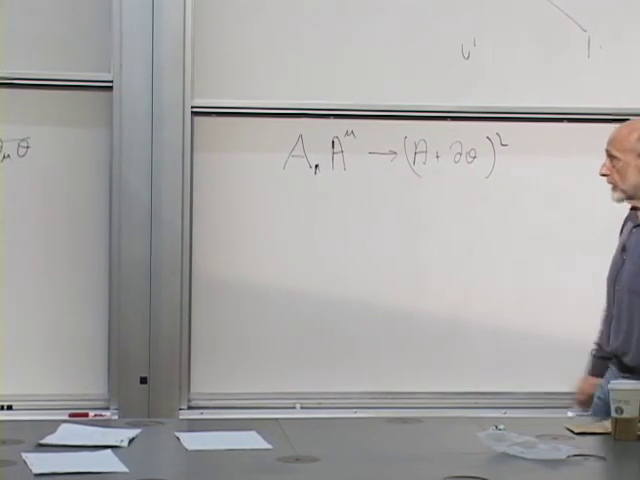
\includegraphics[width=0.76\textwidth]{lecture_08_figure_05.png}
\caption{关于这一阻碍的一个经过验证的板书状态：在规范变换下，\(A_\mu A^\mu\)变成一个包含
\(\partial_\mu\theta\)的平方，因此裸的矢量质量不是不变的。}
\lectureframe{01:07:30}
\label{fig:l08-bare-mass-board}
\end{figure}

\section{希格斯机制}

\subsection{协变导数产生质量}

回到破缺后的势，并使用按正则归一化的参数化
\begin{equation}
  \phi(x)=\frac{f+h(x)}{\sqrt2}
  e^{i\pi(x)/f}.
\end{equation}
其协变导数为
\begin{equation}
  D_\mu\phi
  =
  \frac{e^{i\pi/f}}{\sqrt2}
  \left[
    \partial_\mu h
    +i(f+h)
      \left(\frac{\partial_\mu\pi}{f}+gA_\mu\right)
  \right].
  \label{eq:l08-covariant-polar}
\end{equation}
因此，
\begin{equation}
\begin{aligned}
  (D_\mu\phi)^*D^\mu\phi
  ={}&
  \frac12(\partial_\mu h)^2
  \\
  &+\frac12(f+h)^2
    \left(\frac{\partial_\mu\pi}{f}+gA_\mu\right)
  \\
  &\hspace{4.2em}\times
    \left(\frac{\partial^\mu\pi}{f}+gA^\mu\right).
\end{aligned}
  \label{eq:l08-higgs-kinetic}
\end{equation}

决定性的项在任何规范选择之前就已出现：
\begin{equation}
  \frac12g^2f^2 A_\mu A^\mu.
  \label{eq:l08-vector-mass-term}
\end{equation}
将其与普罗卡形式
\(\frac12m_A^2A_\mu A^\mu\)比较，我们得到
\begin{equation}
  \boxed{m_A=g f}.
  \label{eq:l08-vector-mass}
\end{equation}
同一展开还产生相互作用
\(g^2fh A_\mu A^\mu\)和
\(\frac12g^2h^2A_\mu A^\mu\)。因此，矢量质量并不是对规范对称性的任意破坏。它来自一个规范不变的标量动能项，在平衡量值\(f\)非零的相位中取值。

\begin{figure}[htbp]
\centering
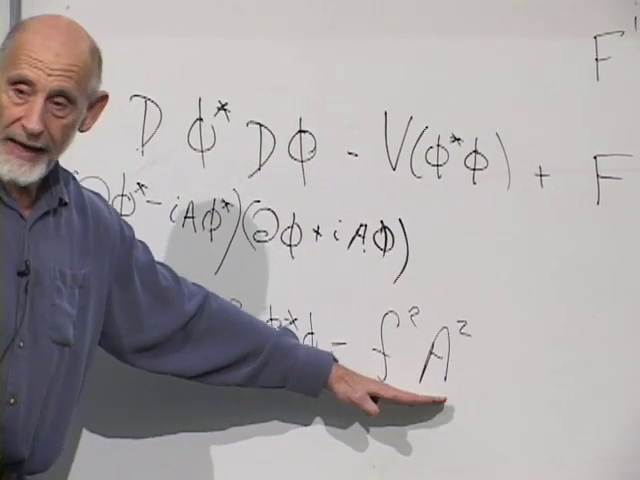
\includegraphics[width=0.78\textwidth]{lecture_08_figure_06.png}
\caption{板书将\(f^2A^2\)贡献分离在
\((D\phi)^*(D\phi)\)之内。数值因子取决于标量场和规范耦合如何归一化；在式~\eqref{eq:l08-canonical-polar}
和\eqref{eq:l08-covariant-convention}下，结果为\(m_A=gf\)。}
\lectureframe{01:10:10}
\label{fig:l08-generated-mass-board}
\end{figure}

讲座将\(g\)和若干\(\sqrt2\)因子吸收进其板书记号，因此在确定质量时，它短暂地在\(f\)、\(2f\)和\(\sqrt2f\)之间交替。在动能项和势的归一化被说明之前，这些因子没有不变的意义。稳健的结果是
\(m_A\propto gf\)；式~\eqref{eq:l08-vector-mass}给出了此处所用约定下的因子。

\subsection{相位被吸收}

在规范变换下，相位变量按如下方式变化：
\begin{equation}
  \pi'(x)=\pi(x)+f\,\theta(x).
\end{equation}
选择
\begin{equation}
  \theta(x)=-\frac{\pi(x)}{f}.
  \label{eq:l08-unitary-gauge-choice}
\end{equation}
于是\(\pi'=0\)。这就是幺正规范，其中
\begin{equation}
  \phi'(x)=\frac{f+h(x)}{\sqrt2}
\end{equation}
为实，而式~\eqref{eq:l08-higgs-kinetic}约化为
\begin{equation}
  (D_\mu\phi')^*D^\mu\phi'
  =
  \frac12(\partial_\mu h)^2
  +\frac12g^2(f+h)^2A_\mu'A^{\prime\mu}.
  \label{eq:l08-unitary-gauge-lagrangian}
\end{equation}
角向戈德斯通场已从独立变量列表中消失，而矢量质量仍然保留。

讲座首先在低能极限\(\rho=f\)下演示这一点，其中
\begin{align}
  \phi&=f e^{i\alpha},
  \notag\\
  D_\mu\phi
  &=if e^{i\alpha}
    \left(\partial_\mu\alpha+gA_\mu\right),
  \notag\\
  (D_\mu\phi)^*
  &=-if e^{-i\alpha}
    \left(\partial_\mu\alpha+gA_\mu\right).
  \label{eq:l08-frozen-radius}
\end{align}
它们的乘积为
\begin{equation}
  f^2
  \left(\partial_\mu\alpha+gA_\mu\right)
  \left(\partial^\mu\alpha+gA^\mu\right).
\end{equation}
选择\(\theta=-\alpha\)后剩下\(g^2f^2A_\mu'A^{\prime\mu}\)。

\begin{figure}[htbp]
\centering
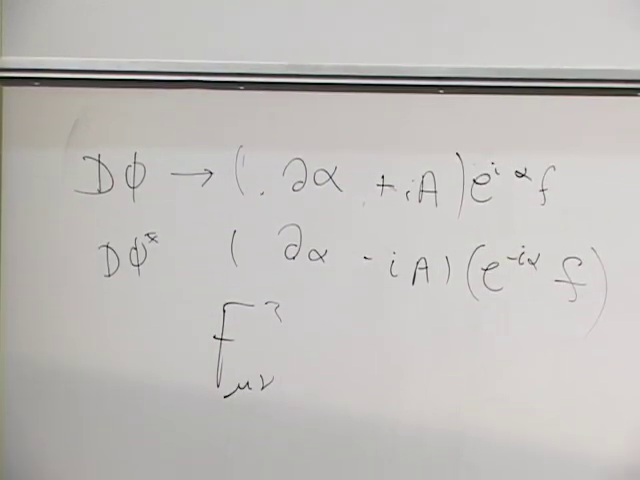
\includegraphics[width=0.82\textwidth]{lecture_08_figure_07.png}
\caption{完整的冻结半径板书状态：协变导数同时包含相位导数和矢量势。讲座接下来选择\(\theta=-\alpha\)，消去相位并留下矢量质量项。}
\lectureframe{01:16:20}
\label{fig:l08-frozen-radius-board}
\end{figure}

\begin{classroomqa}
\audiencequestion{能否将整个拉格朗日量用使角向模消失变得显式的变量重写？
\lecturetimestamp{01:13:49}}
\lecturerresponse{可以。在极坐标变量中，相位仅通过规范不变的组合
\(\partial_\mu\alpha+gA_\mu\)出现。取\(\theta=-\alpha\)的规范变换在该规范定义良好之处处处将相位设为零。标量动能项于是变成矢量质量项，而规范不变的场强项保持不变。}
\end{classroomqa}

\begin{classroomqa}
\audiencequestion{\(\alpha\)中的振荡与规范振荡不可区分吗？\lecturetimestamp{01:18:02}}
\lecturerresponse{在规范理论中，\(\alpha\)的纯粹变化若由\(A_\mu\)的相应变化所补偿，则是一种规范重述，而不是一个不同的物理波。不变量是
\(\partial_\mu\alpha+gA_\mu\)。曾由整体戈德斯通场表示的物理模，重新表现为有质量矢量的纵向极化。}
\end{classroomqa}

人们常说局域规范对称性发生了自发破缺。从操作层面看，这种说法是有用的：选定一个规范后，标量场具有非零真空值，谱中包含一个带质量的矢量。然而严格地说，规范变换联系的是冗余的描述，而不是不同的物理态。\editorialnote{局域规范冗余并不像整体对称性那样以规范不变的意义发生破缺。精确的陈述是，该理论处于希格斯相。规范固定后的微扰论通过非零的标量期望值以及由此产生的带质量矢量谱来描述该相。}

\section{戈德斯通自由度去了哪里}

仅仅因为我们改变了变量，任何物理的东西都不可能消失。数一数进入希格斯相前后的自由度。

之前：
\begin{equation}
  \underbrace{2}_{\text{massless vector}}
  +
  \underbrace{2}_{\text{complex scalar}}
  =4.
\end{equation}
无质量矢量有两个横向极化。复标量有两个实分量，即径向分量和角向分量。

之后：
\begin{equation}
  \underbrace{3}_{\text{massive vector}}
  +
  \underbrace{1}_{\text{radial Higgs}}
  =4.
  \label{eq:l08-degree-count}
\end{equation}
带质量矢量可以被带到静止。在其静止系中没有任何空间方向是特殊的，因此它必须有三个极化态。当它运动时，两个是横向的，一个是纵向的。戈德斯通模变成了那个纵向极化。

\begin{figure}[htbp]
\centering
\begin{adjustbox}{max width=\linewidth}
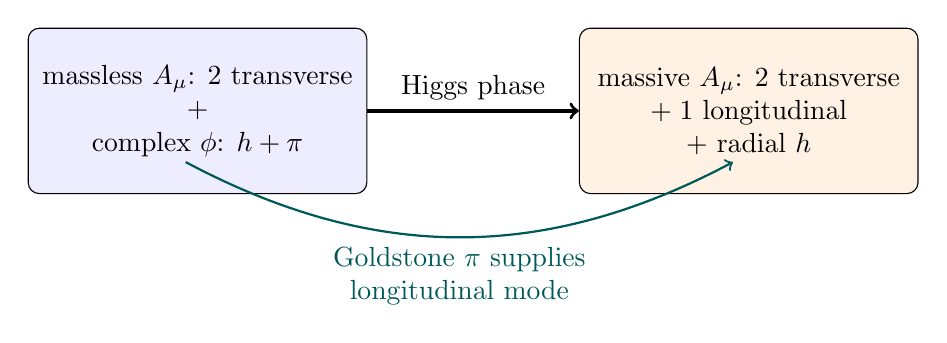
\begin{tikzpicture}[x=1cm,y=1cm]
  \node[draw,rounded corners,fill=blue!7,minimum width=4.3cm,
        minimum height=2.1cm,align=center] (before) at (0,0)
    {massless \(A_\mu\): \(2\) transverse\\
     \(+\)\\
     complex \(\phi\): \(h+\pi\)};
  \node[draw,rounded corners,fill=orange!10,minimum width=4.3cm,
        minimum height=2.1cm,align=center] (after) at (7,0)
    {massive \(A_\mu\): \(2\) transverse\\
     \(+\;1\) longitudinal\\
     \(+\) radial \(h\)};
  \draw[->,very thick] (before) -- node[above]{Higgs phase} (after);
  \draw[->,teal!70!black,thick]
    (-0.15,-0.65) to[bend right=28]
    node[below,align=center]{Goldstone \(\pi\) supplies\\longitudinal mode}
    (6.8,-0.65);
\end{tikzpicture}
\end{adjustbox}
\caption{希格斯机制重新排列而不是消灭物理自由度。}
\label{fig:l08-degree-rearrangement}
\end{figure}

\begin{classroomqa}
\audiencequestion{角向自由度怎么可能在不违反自由度计数的前提下消失？\lecturetimestamp{01:19:13}}
\lecturerresponse{它在物理上并没有消失。无质量矢量有两个螺旋度，因为它不能被带到静止。带质量矢量有三个极化，其中包括一个纵向极化。戈德斯通模变成了那第三个极化，从而使总数保持不变。}
\end{classroomqa}

讲座提供了一个有用的运动学检验。想象一个带质量的矢量粒子，把它减速到静止，再沿一个新方向加速它。相对于原来的运动为横向的极化，相对于新的运动可以变成纵向的。同样，如果一个圆极化的带质量粒子被带着经过静止并沿相反方向发出，它的螺旋度标签会反转。严格无质量的粒子不能经历这个实验，因为没有任何惯性系能把它带到静止。因此它的两个螺旋度构成一个自洽的物理谱。

\section{超导类比}

在常规超导体中，电子形成库珀对。一个对是携带电荷\(2e\)的玻色子，凝聚体由一个带电的复序参量描述。当其幅度非零时，其相位与电磁矢量势的组合产生安德森--希格斯机制。静磁场在伦敦穿透深度内衰减，而不是自由地延伸到体内。在这种精确的、依赖于介质的含义下，光子表现得好像获得了质量。

这个例子也澄清了开头的区分。电磁场并没有永久地转变成一种不同的基本粒子。带质量的传播规律属于材料内部的集体态；在外部，真空光子仍然是无质量的。

\section{已经确立了什么}

现在可以在不丢失其逻辑的情况下压缩这一论证：
\begin{enumerate}
  \item 破缺的整体连续对称性有一个平坦的角向方向，因此有一个无质量的戈德斯通模。
  \item 局域相位不变性要求一个规范势，并把\(\partial_\mu\)替换为\(D_\mu\)。
  \item 裸的\(A_\mu A^\mu\)质量违反局域变换律。
  \item 当带电标量具有非零平衡幅度\(f\)时，规范不变项\(|D_\mu\phi|^2\)包含\(\frac12g^2f^2A_\mu A^\mu\)。
  \item 通过选择规范可以去掉相位，其物理自由度变成带质量矢量的纵向极化。
  \item 径向希格斯激发仍然存在，其质量由标量势的曲率固定。
\end{enumerate}

下一个任务是赋予费米子质量。电子和夸克不能直接使用矢量机制；它们与希格斯的耦合是汤川相互作用。一旦标量稳定在\(f\)，这些相互作用就变成费米子质量项。

“若无电弱对称性破缺，我们熟悉的粒子将没有质量”这一宽泛论断还需要最后一项限定。基本夸克与带电轻子的质量，以及\(W\)和\(Z\)的质量，确实会随希格斯期望值而消失。然而，质子和中子的大部分质量并非来自夸克的希格斯质量，而是由QCD禁闭和强场能量动力学地产生。这一区分并不改变此处推导出的希格斯机制；它只是使该机制的适用范围保持精确。